% !TEX root = ../main.tex
\chapter{Tests de Cuanticidad y Mapeos Cuántico-Compatibles}
\label{cap:investigacion_original}

Los capítulos anteriores han mostrado un patrón consistente: la ventaja cuántica en kernels aparece con robustez cuando el \textbf{generador del dato está alineado con el feature map} del kernel ---en los experimentos de este TFM, datos sintéticos generados con el \texttt{ZZFeatureMap} de modo que ese kernel es óptimo por construcción---, y desaparece en datos reales de movilidad y telecomunicaciones sin esa alineación. ZZ no es el único mapa posible (Pauli, IQP, re-uploading, etc.); es el que se validó empíricamente aquí. Este resultado plantea dos preguntas que este capítulo aborda como contribución original del TFM:

\begin{enumerate}
    \item \textbf{Tests de cuanticidad}: \textquestiondown{}Existe algún indicador calculable a priori sobre un dataset que permita predecir si un algoritmo cuántico mostrará ventaja sobre los clásicos?
    \item \textbf{Mapeos cuántico-compatibles}: Si un dataset no tiene estructura cuántica nativa, \textquestiondown{}puede transformarse a un espacio de representación donde la tenga, sin alterar la información discriminativa?
\end{enumerate}

Ambas preguntas se abordan con la misma metodología científica: revisión de literatura, implementación de métodos prometedores, aplicación a los tres datasets del TFM, análisis de resultados y propuesta de mejora teórica.

% =====================================================================
\section{Tests de cuanticidad: revisión de la literatura}
\label{sec:lit_cuanticidad}
% =====================================================================

\subsection{El problema de la selección de algoritmo a priori}

El problema de seleccionar el algoritmo más adecuado antes del entrenamiento es un problema clásico en aprendizaje automático, tratado bajo el marco del \textit{No Free Lunch Theorem} \citep{wolpert1997}. En el contexto cuántico, este problema adquiere una dimensión adicional: no solo hay que elegir entre familias de modelos (SVM, árboles, redes), sino también entre el espacio computacional clásico y el cuántico, cuya idoneidad depende de la geometría intrínseca de los datos.

\subsection{Kernel alignment como indicador de alineación estructural}

El \textit{kernel alignment} \citep{cortes2012} es una medida de la correspondencia entre la geometría inducida por un kernel y la estructura de clases de un dataset. Formalmente, dado un kernel $K$ y la matriz de etiquetas $K_y = yy^T$, se define:

\begin{equation}
    A(K, K_y) = \frac{\langle K, K_y \rangle_F}{\|K\|_F \cdot \|K_y\|_F}
    \label{eq:kernel_alignment}
\end{equation}

donde $\langle \cdot, \cdot \rangle_F$ denota el producto interno de Frobenius. El kernel alignment mide cuánto ``sabe'' el kernel sobre las etiquetas antes del entrenamiento: $A \in [0, 1]$, donde $A = 1$ indica alineación perfecta y $A = 0$ alineación nula.

\citet{huang2021} adaptaron este concepto al contexto cuántico, proponiendo el \textit{geometric difference} $g(K_Q, K_{cl})$ como medida de la separación entre los espacios de características cuántico y clásico. Su resultado teórico central acota el error de predicción de un modelo de kernel mediante su complejidad $s_K(N)$ y establece que, si $g$ es pequeña, un modelo clásico tiene una complejidad, y por tanto un error de predicción, similar o mejor que el cuántico, con independencia de las etiquetas. Una $g$ grande es solo una condición necesaria: garantiza que existe un conjunto de etiquetas con ventaja cuántica, no que el dataset real la tenga.

\begin{figure}[ht]
\centering
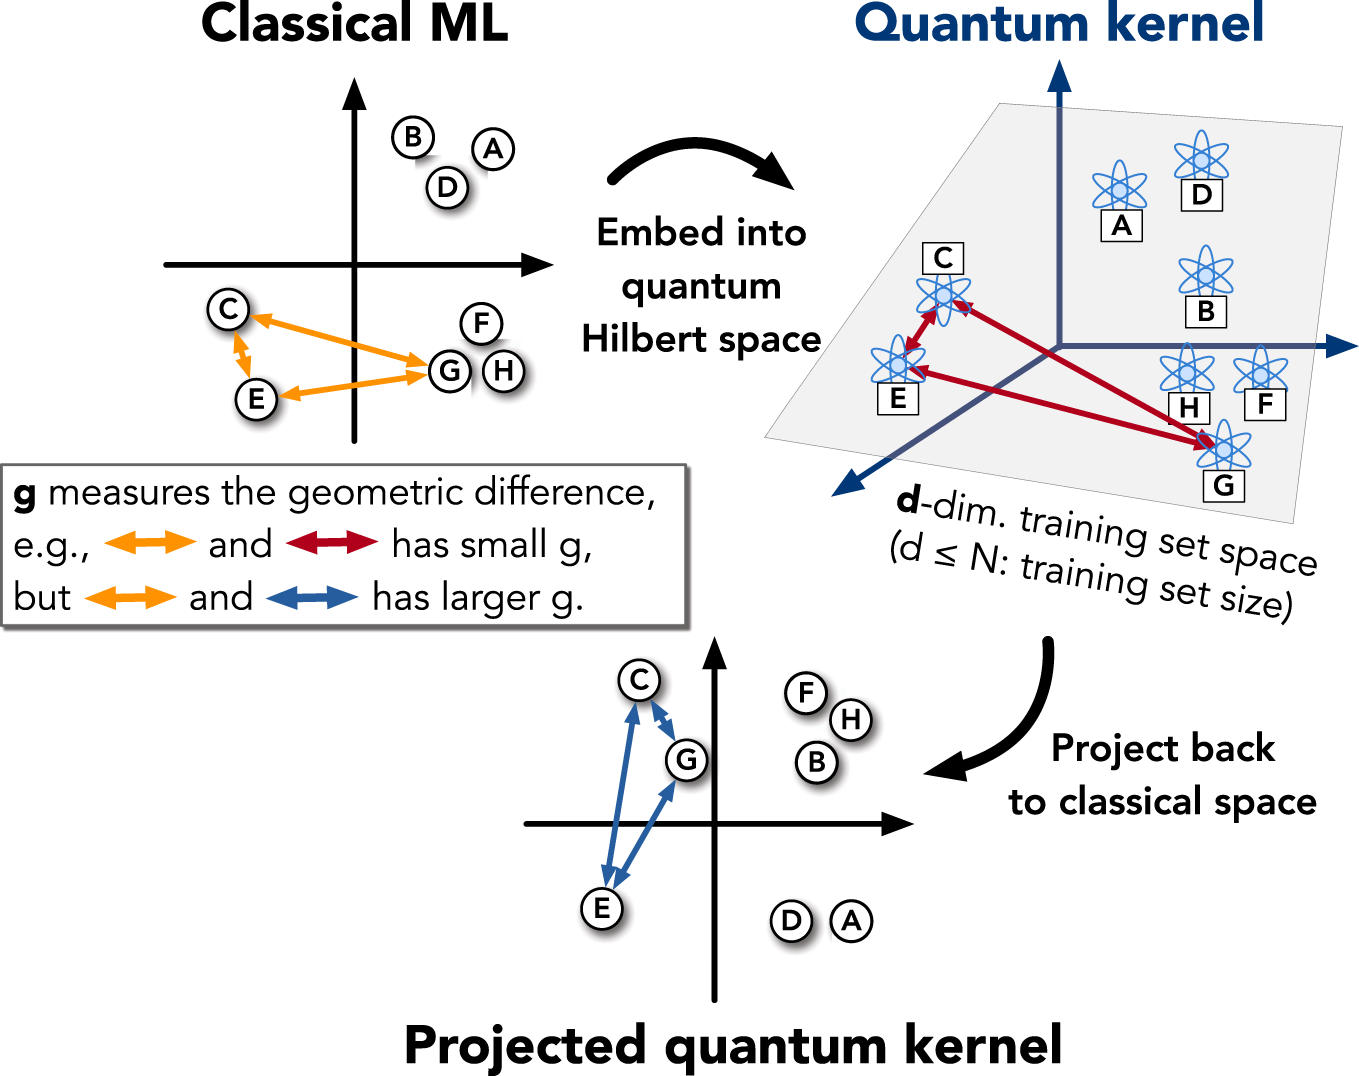
\includegraphics[width=0.62\textwidth]{Imagenes/huang2021_fig2_geometria_kernel.png}
\caption{Geometría del kernel clásico y cuántico. Las letras A, B, \dots{} son puntos de datos $\{x_i\}$ en espacios distintos; las flechas representan la similitud (función kernel) entre datos. La diferencia geométrica $g$ compara las similitudes entre modelos (flechas naranja/roja: $g$ pequeño; naranja/azul: $g$ mayor) y $d$ es una dimensión efectiva del conjunto de datos en el espacio de Hilbert cuántico. Reproducida de \citet{huang2021}, Fig.~2, bajo licencia CC~BY~4.0.}
\label{fig:huang_geometria}
\end{figure}

\subsection{Concentración exponencial y entropía espectral}

\citet{thanasilp2022} identificaron que los kernels cuánticos exhiben \textit{concentración exponencial} bajo cuatro condiciones: alta expresividad del mapa de datos, mediciones globales, entrelazamiento excesivo y ruido. La concentración implica que todos los valores del kernel convergen a una constante, lo que destruye la información discriminativa.

Un indicador directo de concentración es la \textbf{entropía espectral} de la matriz de Gram $K_Q$. Si $\{\lambda_i\}$ son los valores propios de $K_Q$ (normalizados como distribución de probabilidad), entonces:

\begin{equation}
    H(K_Q) = -\sum_{i} \hat{\lambda}_i \log \hat{\lambda}_i, \quad \hat{\lambda}_i = \frac{\lambda_i}{\sum_j \lambda_j}
    \label{eq:spectral_entropy}
\end{equation}

Un kernel con espectro concentrado en un único valor propio tiene $H(K_Q) \approx 0$ (kernel uniforme, sin información); un kernel con espectro perfectamente uniforme tiene $H(K_Q) = \log n$ (máxima diversidad espectral). La hipótesis es que datasets con ventaja cuántica exhiben $H(K_Q) \gg H(K_{RBF})$.

\subsection{Divergencia cuántica-clásica en el espacio de kernels}

\citet{liu2021} demostraron, bajo la conjetura de dificultad del logaritmo discreto, que existe un problema de clasificación que un kernel cuántico aprende de forma eficiente y que ningún algoritmo clásico eficiente puede aprender. De ahí se desprende que una ventaja de este tipo exige un kernel difícil de aproximar clásicamente. Un proxy operativo, definido en este trabajo y no propuesto por esos autores, es la \textbf{distancia de Frobenius normalizada}:

\begin{equation}
    d_F(K_Q, K_{cl}) = \frac{\|K_Q - K_{cl}^*\|_F}{n}
    \label{eq:frobenius_dist}
\end{equation}

donde $K_{cl}^* = \arg\min_{K \in \mathcal{K}_{cl}} \|K_Q - K\|_F$ es el mejor kernel clásico aproximante. En la práctica, $K_{cl}^*$ se aproxima buscando el mejor $\sigma$ del kernel RBF. Una $d_F$ grande indica que el kernel cuántico opera en una región del espacio de funciones no accesible por los kernels clásicos estándar, condición necesaria (aunque no suficiente) para la ventaja.

\subsection{Métricas de expresividad del circuito}

\citet{sim2019} definieron la \textit{expressibility} de un ansatz cuántico como la capacidad de sus estados para explorar el espacio de Hilbert. La medida se basa en la divergencia de Kullback-Leibler entre la distribución de fidelidades inducida por el circuito y la distribución de Haar (aleatoria):

\begin{equation}
    \text{Expr} = D_{KL}(\hat{P}_{PQC}(F; \theta) \,\|\, P_{Haar}(F))
    \label{eq:expressibility}
\end{equation}

Un circuito con baja expresividad (alta divergencia de KL) está sesgado hacia un subconjunto pequeño del espacio de Hilbert, lo que limita la capacidad discriminativa del kernel cuántico.

\subsection{Cota de ventaja basada en datos (Huang et al., 2021)}

\citet{huang2021} propusieron un diagrama de decisión para evaluar la ventaja potencial de un modelo cuántico con un número fijo de datos de entrenamiento. Dado un kernel $K$ y $N$ datos, el error de predicción está acotado por $c\sqrt{s_K(N)/N}$, donde $s_K(N)=\lVert w\rVert^2$ es la complejidad del modelo entrenado. Para dos kernels $K_1$ y $K_2$ con $\mathrm{Tr}\,K_1=\mathrm{Tr}\,K_2=N$ se cumple

\begin{equation}
    s_{K_1}(N) \leq g(K_1\Vert K_2)^2\, s_{K_2}(N),
    \qquad
    g(K_1\Vert K_2)=\sqrt{\bigl\lVert \sqrt{K_2}\,K_1^{-1}\sqrt{K_2}\bigr\rVert_\infty},
    \label{eq:huang_bound}
\end{equation}

de modo que, si $g(K_C\Vert K_Q)$ es pequeña, el modelo clásico es competitivo o mejor que el cuántico. Si es grande, existe un conjunto de etiquetas para el que el modelo cuántico predice mejor, pero eso no implica que ocurra en un dataset concreto. Este resultado liga los indicadores de geometría de kernels con cotas de error de predicción, y es la base teórica de la diferencia geométrica $g$ usada en este trabajo; no es un test estadístico de significación.

% =====================================================================
\section{Resultados prometedores de la literatura}
\label{sec:lit_resultados}
% =====================================================================

La Tabla~\ref{tab:lit_indicadores} resume los indicadores propuestos en la literatura, su fundamento teórico, su complejidad computacional y su conexión con la ventaja cuántica demostrada.

\begin{table}[ht]
\centering
\small
\begin{tabular}{>{\raggedright\arraybackslash}p{3.1cm}>{\raggedright\arraybackslash}p{2.7cm}>{\raggedright\arraybackslash}p{2.5cm}>{\raggedright\arraybackslash}p{4.0cm}}
\hline
\textbf{Indicador} & \textbf{Base conceptual} & \textbf{Complejidad} & \textbf{Relación con la literatura} \\
\hline
Kernel alignment $A(K_Q, K_y)$ & \citet{cortes2012, huang2021} & $O(n^2)$ & Mide el ajuste kernel--etiquetas; no es por sí sola condición de ventaja \\
Entropía espectral $H(K_Q)$ & \citet{thanasilp2022} & $O(n^3)$ & Proxy propio de la concentración del kernel descrita por esos autores \\
Distancia Frobenius $d_F$ & \citet{liu2021} & $O(n^2)$ & Proxy propio de la dificultad de aproximación clásica \\
Diferencia geométrica $g$ & \citet{huang2021} & $O(n^2)$ & Aparece en la cota $s_{K_1}\leq g^2 s_{K_2}$ de la Ec.~\ref{eq:huang_bound} \\
Expressibility & \citet{sim2019} & $O(2^n)$ & Capacidad de exploración del espacio de Hilbert \\
\hline
\end{tabular}
\caption{Indicadores de cuanticidad propuestos en la literatura, con su referencia original, complejidad y base teórica.}
\label{tab:lit_indicadores}
\end{table}

La literatura \citep{huang2021, thanasilp2022, schuld2021kernels} indica que ningún indicador individual es condición suficiente para la ventaja; la combinación de $A(K_Q, K_y) > A(K_{cl}, K_y)$ (el kernel cuántico está más alineado con las etiquetas) y $d_F > \epsilon$ (el kernel cuántico es genuinamente diferente del clásico) es la combinación que se adopta como criterio operativo en este trabajo.

% =====================================================================
\section{Aplicación a los datasets del TFM}
\label{sec:aplicacion_cuanticidad}
% =====================================================================

Se implementaron los cinco indicadores anteriores sobre los tres datasets del TFM utilizando el Notebook~08 (\texttt{08\_test\_cuanticidad\_datasets.ipynb}). Para cada dataset se calculó la matriz de kernel cuántico $K_Q$ (ZZFeatureMap, 2 qubits, tras reducción PCA a 2 dimensiones) y la mejor matriz de kernel clásico $K_{RBF}^*$ (búsqueda de $\sigma$ óptimo por validación cruzada).

\subsection{Resultados cuantitativos}

\begin{table}[ht]
\centering
\small
\begin{tabular}{lccccccc}
\hline
\textbf{Dataset} & $A(K_Q,K_y)$ & $A(K_{cl},K_y)$ & $H(K_Q)$ & $H(K_{cl})$ & $d_F$ & $\Delta_{\mathrm{RBF}}$ & \textbf{$\Delta_{\mathrm{op}}$} \\
\hline
Cuántico-nativo  & 0.027 & 0.056 & 2.307 & 3.427 & 0.358 & $+4.2$ & $\mathbf{+8.9}$ \\
SKG Incidentes   & 0.040 & 0.050 & 2.155 & 1.967 & 0.369 & $+8.3^\dagger$ & $\mathbf{-4.0}$ \\
Telco Churn      & 0.190 & 0.170 & 2.333 & 3.465 & 0.346 & $+$0.0 & $\mathbf{-3.8}$ \\
\hline
\end{tabular}
\caption{Indicadores de cuanticidad (Notebook~08, ZZFeatureMap 2~qubits, PCA~2D, $n=80$). Geometría vs.\ kernel clásico de referencia; $\Delta_{\mathrm{RBF}}$ = QSVM$-$SVM-RBF en el split NB08 (baseline débil). Columna $\Delta_{\mathrm{op}}$ = accuracy(QSVM)$-$accuracy(\textbf{mejor clásico}) en \textbf{clasificación} (Notebook~06): nativo $+8.9$~pp, SKG $-4.0$~pp, Telco $-3.8$~pp vs Gradient Boosting --- no es una métrica geométrica. Los indicadores del dataset nativo dependen del etiquetado por autovector del kernel, que es sensible al \emph{backend} numérico (véase la nota siguiente). $^\dagger$SKG $+8.3$~pp vs RBF es artefacto ---bajo $\mathcal{Q}_{\mathrm{rob}}$ y frente al stack clásico SKG es \texttt{classical}.}
\label{tab:indicadores_resultados}
\end{table}

\paragraph{Sensibilidad numérica del dataset nativo.}
En el Notebook~08 las etiquetas del dataset nativo se definen por el signo de un autovector de $K_Q$, elección que es inestable cuando hay autovalores casi degenerados. Al reejecutar el cuaderno de principio a fin (Qiskit~2.6.1, NumPy~2.5) los indicadores de ese dataset cambiaron respecto a la ejecución original ($\Delta H$ de $+0.034$ a $-1.120$, $\mathcal{Q}$ de $+0.286$ a $-0.056$, $\Delta_{\mathrm{RBF}}$ de $0.0$ a $+4.2$~pp), mientras que SKG, Telco y el barrido $\alpha$ se reprodujeron exactamente. La tabla recoge las cifras reejecutadas; la conclusión es que $\Delta H$ y $\mathcal{Q}$ del dataset nativo \textbf{no} son estables frente al entorno numérico y no deben leerse como una propiedad del dataset.

\subsection{Figuras de resultados}

\begin{figure}[ht]
\centering
\includegraphics[width=0.95\textwidth]{../POCs/data/output/figures/08_test_cuanticidad_datasets.png}
\caption{Perfil vectorial $\mathcal{Q}(\mathcal{D})=(\Delta A,d_F,\Delta H)$ sobre los tres datasets (Notebook~08). Fila superior: componentes del vector. Fila inferior: alineaciones, entropías de apoyo y el escalar ponderado $w^\top\mathcal{Q}$ (experimento; \textbf{no} regla de adopción). Telco y nativo dominados por $\Delta H$ ($-1.131$ y $-1.120$). La decisión operativa usa $\Delta_{\mathrm{op}}$ (Tabla~\ref{tab:indicadores_resultados}), no el escalar.}
\label{fig:indicadores_cuanticidad}
\end{figure}

\paragraph{Nota sobre visuales de matrices de kernel.}
Las matrices $K_Q$/$K_{cl}$ viven en memoria durante la ejecución del Notebook~08 y \textbf{no se serializaron} como artefactos. Un heatmap o ``contraste de bloques'' regenerado a posteriori (sin re-ejecutar el notebook) sería construcción ilustrativa, no medición. Por criterio de este TFM (\emph{nada forzado ni construido a mano}) esa figura se \textbf{retira} del cuerpo; la geometría se reporta solo vía los indicadores tabulares ($d_F$, $g$, $\Delta A$, $\Delta H$).

\subsection{Análisis: \textquestiondown{}Predicen los indicadores la ventaja QSVM?}

La Tabla~\ref{tab:indicadores_resultados} distingue dos rankings. Bajo el protocolo NB08 vs.\ un baseline RBF débil: SKG ($+8.3$~pp) $>$ nativo ($+4.2$~pp) $>$ Telco ($0.0$~pp) ---ranking \textbf{engañoso}. El ranking operativo vs.\ mejor clásico es: \textbf{nativo ($+8.9$~pp)} $>$ Telco ($-3.8$~pp) $>$ SKG ($-4.0$~pp). Solo el régimen cuántico-nativo muestra ventaja; SKG/Telco son clásicos (Sección~\ref{sec:qml_v2_revision}).

El score $\mathcal{Q}(\mathcal{D})$ (calculado vs.\ kernel clásico de referencia) ordena SKG ($+0.352$) $>$ Telco ($-0.050$) $>$ nativo ($-0.056$): el único dataset con ventaja operativa queda el último. Frente al ranking vs.\ RBF la relación es débil ($\rho_S=+0.5$, $n=3$) y frente al ranking operativo es inversa ($\rho_S=-1.0$ entre $\mathcal{Q}$ y $\Delta_{\mathrm{op}}$, $n=3$): en esta implementación, con 2 qubits y PCA a 2 dimensiones, $\mathcal{Q}$ \textbf{no} identifica el régimen nativo. El barrido sintético NB08 ($n=9$, $X$ fijo + mezcla de etiquetas) muestra $\rho_S(\alpha,\Delta A)=+0.833$ ($p=0.005$): resultado esperable por construcción, ya que mezclar etiquetas cuánticas aumenta la alineación con el kernel. Bajo ese protocolo $d_F$ y $H$ son constantes, y $\rho_S(\alpha,\mathrm{ventaja})\approx 0.34$ (n.s.) ---\textbf{no} se afirma que $\mathcal{Q}$ prediga ventaja con $\rho=0.833$. Lectura: $\mathcal{Q}>0$ vs.\ un baseline débil \textbf{no} autoriza desplegar el módulo cuántico.

El análisis individual de los componentes revela matices importantes:
\begin{itemize}
    \item $\Delta A$ es negativa en dos de los tres datasets en el régimen 2~qubits + PCA. Frente a $\Delta_{\mathrm{op}}$, $\rho_S(\Delta A,\Delta_{\mathrm{op}})=-0.500$ ($n=3$); en el barrido NB08 $\rho_S(\alpha,\Delta A)=+0.833$: el PCA agresivo suprime la señal de $\Delta A$ en datos reales.
    \item $d_F$ y $g$ frente a $\Delta_{\mathrm{op}}$ dan $\rho_S=-0.5$ y $-1.0$ ($n=3$): no sustituyen la comparación contra el mejor clásico ni el veredicto $\mathcal{Q}_{\mathrm{rob}}$.
    \item $\Delta H$ es el indicador más volátil: $\mathcal{Q}$ de Telco y del nativo están dominados por $\Delta H=-1.131$ y $-1.120$ (concentración espectral).
\end{itemize}

\paragraph{Caveat estadístico.}
Con $n=3$ datasets, cualquier $\rho_S$ es de potencia baja (máximo $\pm 1$ o $\pm 0.5$ con empates). El $\rho_S=+0.833$ del barrido es $\rho(\alpha,\Delta A)$, no $\rho(\mathcal{Q},\mathrm{ventaja})$. La validación sobre más datasets y un barrido structure-aware (donde $d_F$/$H$ también varíen) es trabajo futuro explícito (Capítulo~\ref{cap:futuro}).

\paragraph{Debilidades metodológicas expuestas (integridad de resultados).}
Un buen TFM se discute desde lo medido, no desde lo deseable. Aquí se exponen límites \textbf{sin alterar cifras}:
\begin{itemize}
    \item Barrido $\alpha$ con $X$ fijo: $d_F$, $H$ y $g$ constantes ---no valida monotonía de todos los factores de $\mathcal{Q}$.
    \item Ventaja NB08 vs.\ RBF en SKG ($+8.3$~pp) es artefacto de baseline débil; el $\Delta_{\mathrm{op}}$ viene de otro protocolo (Caso~1 / NB06) y \textbf{no} se mezcla en la misma $\rho$.
    \item $n=3$ no sostiene correlaciones fuertes entre $\mathcal{Q}$ y ventaja operativa.
    \item No hay dumps de $K$ en artefactos: no se inventan heatmaps.
    \item Series de rotación NB09: PNG del notebook; no regenerar con curvas proxy.
    \item Componentes $\Delta A$/$d_F$/$\Delta H$ \emph{post} re-uploading no están en el log NB09: no se inventan (solo $Q$ y Adv post están verificados).
\end{itemize}

\begin{figure}[ht]
\centering
\includegraphics[width=0.92\textwidth]{../POCs/data/output/figures/08_barrido_sintetico_alpha.png}
\caption{Barrido sintético NB08 (datos reales): $\alpha$ = fracción de etiquetas cuánticas con $X$ fijo. $\Delta A$ crece con $\alpha$ ($\rho_S=+0.833$, $p=0.005$). $d_F$ y $H(K_Q)$ son constantes por diseño (los kernels no dependen de las etiquetas). La ventaja supervisada es ruidosa ($\rho_S(\alpha,\mathrm{ventaja})\approx 0.34$). El número $0.833$ es $\rho(\alpha,\Delta A)$, \textbf{no} $\rho(\mathcal{Q},\mathrm{ventaja})$.}
\label{fig:barrido_sintetico_alpha}
\end{figure}

\begin{figure}[!htbp]
\centering
\includegraphics[width=0.88\textwidth]{../POCs/data/output/figures/08_correlacion_indicadores_ventaja.png}
\caption{Indicadores NB08 vs.\ ventaja NB08 (QSVM$-$SVM-RBF, puntos rellenos). Marcadores huecos: $\Delta_{\mathrm{op}}$ de Caso~1/NB06 (referencia; \textbf{no} entran en $\rho$). Línea gris: barrido $\alpha$ solo en el panel $\Delta A$ (único factor que varía con $X$ fijo). $n=3$: potencia baja; no se reclama $\rho(\mathcal{Q},\mathrm{ventaja})=0.833$.}
\label{fig:correlacion_indicadores_body}
\end{figure}

\subsection{Análisis de sensibilidad: impacto de la reducción dimensional}

Un hallazgo metodológico relevante emerge al comparar la configuración base (2 qubits + PCA 2D) con una configuración alternativa (4 qubits + SelectKBest por información mutua). Con 2 qubits + PCA, la varianza explicada es del $31.8\%$ en SKG y $30.7\%$ en Telco. La Tabla~\ref{tab:sensibilidad_dim} muestra que aumentar a 4 qubits con selección de features discriminativas \emph{reduce} $\mathcal{Q}(\mathcal{D})$ en ambos datasets.

\begin{table}[ht]
\centering
\small
\begin{tabular}{llcccc}
\hline
\textbf{Dataset} & \textbf{Config.} & $\mathcal{Q}(\mathcal{D})$ & $\Delta A$ & $d_F$ & \textbf{$\Delta$ vs RBF} \\
\hline
SKG Incidentes & 2Q + PCA       & $+0.352$ & $-0.010$ & $0.369$ & $+8.3$ pp$^\dagger$ \\
               & 4Q + SelectKBest & $-0.128$ & $-0.033$ & $0.197$ & $+8.3$ pp$^\dagger$ \\
Telco Churn    & 2Q + PCA       & $-0.050$ & $+0.020$ & $0.346$ & $+0.0$ pp \\
               & 4Q + SelectKBest & $-0.155$ & $+0.055$ & $0.234$ & $-4.2$ pp \\
\hline
\end{tabular}
\caption{Sensibilidad dimensional (Notebook~08, §11). Columna $\Delta$ vs RBF $=$ QSVM$-$SVM-RBF del protocolo NB08 (\textbf{no} $\Delta_{\mathrm{op}}$). $^\dagger$SKG $+8.3$~pp vs RBF es artefacto: operativo $-4.0$~pp y $\mathcal{Q}_{\mathrm{rob}}$ da \texttt{classical}. Con SelectKBest, $d_F$ (y $\mathcal{Q}$) caen porque el clásico aprovecha mejor features discriminativas.}
\label{tab:sensibilidad_dim}
\end{table}

La interpretación es que el \texttt{ZZFeatureMap} captura mejor la cuanticidad cuando los datos tienen baja información mutua con la clase (como las primeras componentes PCA), porque en ese caso el kernel clásico RBF también rinde mal y $d_F$ es alto. Features altamente informativas permiten que el clasificador clásico mejore más que el cuántico. Este hallazgo implica que $\mathcal{Q}(\mathcal{D})$ debe interpretarse siempre en el contexto de la reducción dimensional aplicada: mide la cuanticidad del subespacio proyectado, no del dataset completo.

% =====================================================================
\section{Propuesta teórica: perfil (vector) de cuanticidad}
\label{sec:score_cuanticidad}
% =====================================================================

Sobre la base de la literatura y la evidencia empírica, se propone tratar la cuanticidad como un \textbf{vector de métricas} que se inspecciona componente a componente ---no como un único escalar de decisión:

\begin{equation}
    \mathcal{Q}(\mathcal{D})
    \;=\;
    \bigl(\Delta A,\; \hat{d}_F,\; \Delta H,\; \hat{g}\bigr)
    \label{eq:score_cuanticidad}
\end{equation}

donde:
\begin{itemize}
    \item $\Delta A = A(K_Q, K_y) - A(K_{RBF}, K_y)$: diferencia de alineación cuántica vs.\ clásica
    \item $\hat{d}_F = d_F / d_{F,\mathrm{ref}}$: distancia de Frobenius normalizada (aquí, respecto al máximo entre datasets del protocolo)
    \item $\Delta H = H(K_Q) - H(K_{RBF})$: diferencia de entropía espectral
    \item $\hat{g} = g / g_{\mathrm{ref}}$: diferencia geométrica de \citet{huang2021},
    \[ g=\sqrt{\bigl\|\sqrt{K_Q}\,(K_{RBF}+\lambda I)^{-1}\sqrt{K_Q}\bigr\|_2}, \]
    con kernels normalizados a $\mathrm{Tr}\,K=n$ y $\lambda=10^{-3}$; normalizada por el máximo entre casos del protocolo, igual que $\hat d_F$. Mide cuánto \emph{no} reproduce el RBF la geometría del kernel cuántico: es condición necesaria, no suficiente, de ventaja, y no usa $y$.
\end{itemize}

Puede ampliarse con otras entradas ($\Delta_{\mathrm{op}}$, veredicto $\mathcal{Q}_{\mathrm{rob}}$, etc.). La lectura es la de un \emph{perfil}: p.~ej.\ Telco muestra cuello en $\Delta H$; SKG puede tener $\hat{d}_F$ alto y aun así $\Delta_{\mathrm{op}}<0$.

\paragraph{Por qué no colapsar a un escalar $w^\top\mathcal{Q}$.}
En el Notebook~08 se calculó también $q=w_1\Delta A+w_2\hat{d}_F+w_3\Delta H$ con pesos fijos $(0.4,0.3,0.3)$; con $\hat g$ como cuarto término la convención del protocolo unificado es $\mathcal{Q}_{\mathrm{comp}}=0.4\,\Delta A+0.2\,\hat d_F+0.2\,\Delta H+0.2\,\hat g$ (se conserva $0.4$ para $\Delta A$ y el resto se reparte a partes iguales; es una convención, no un ajuste). Ese escalar mezcla escalas distintas ($\hat{d}_F\!\approx\!1$ empuja $q>0$ aunque $\Delta A<0$; $\Delta H$ puede dominar) y \textbf{ordena mal} frente a $\Delta_{\mathrm{op}}$: SKG maximiza $q$ ($+0.35$) con $\Delta_{\mathrm{op}}=-4.0$~pp. Por criterio de este TFM, el escalar \textbf{no} se usa como regla de adopción; se conserva solo como experimento negativo. La forma útil de $\mathcal{Q}(\mathcal{D})$ es el \textbf{vector}.

\begin{figure}[ht]
\centering
\includegraphics[width=0.95\textwidth]{../POCs/data/output/figures/08_estructura_comparativa_casos_uso.png}
\caption{Comparativa de estructura cuántica en un solo gráfico: \textbf{un panel por indicador} ---alineación $\Delta A$, entropía espectral $\Delta H$, distancia de Frobenius $d_F$, diferencia geométrica $g$ y compuesto $\mathcal{Q}$, los indicadores de la Tabla de indicadores implementados---; en cada panel el eje X son los \textbf{casos de uso} (clasificación, regresión, anomalías y optimización) y las tres barras de cada grupo son los datasets (Nativo / SKG / Referencia; en optimización, asignación / MaxCut / TSP). Protocolo unificado (ZZ 2~qubits, $n{=}60$, 3 repeats, RBF Frobenius-best). En optimización, $\Delta H$, $d_F$ y $g$ dependen solo del número de bits (asignación y TSP comparten $X$ y $K_Q$); lo que distingue un problema de otro es $\Delta A$. $X$ son todos los bitstrings del espacio de búsqueda e $y$ la energía del QUBO (paisaje), \emph{no} el rendimiento de QAOA. La banda azul del panel de $\Delta A$ es el control nulo ($y$ permutada, $\pm2\sigma$). Solo los nativos superan el ruido de $\Delta A$; $\Delta H$, $d_F$ y $g$ quedan casi planos, con la excepción de anomalías-SKG, atribuible a que los outliers a $8\sigma$ comprimen el escalado MinMax de los inliers (artefacto de codificación). $\mathcal{Q}=0.4\,\Delta A+0.2\,\hat d_F+0.2\,\Delta H+0.2\,\hat g$ (con $\hat d_F=d_F/\max d_F$ y $\hat g=g/\max g$) lo dominan indicadores planos: se muestra por completitud, no como regla de decisión. CSV: \texttt{estructura\_por\_caso\_uso.csv}; notebook~11.}
\label{fig:estructura_tres_casos}
\label{fig:q_vector_vs_nativo}
\end{figure}

\begin{figure}[ht]
\centering
\includegraphics[width=0.85\textwidth]{../POCs/data/output/figures/08_perfil_clasificacion.png}
\caption{Detalle \textbf{clasificación} (todos los datasets de la familia). Auxiliar a la Fig.~\ref{fig:estructura_tres_casos}.}
\label{fig:perfil_clasificacion}
\end{figure}

\begin{figure}[ht]
\centering
\includegraphics[width=0.85\textwidth]{../POCs/data/output/figures/08_perfil_regresion.png}
\caption{Detalle \textbf{regresión}. Auxiliar a la Fig.~\ref{fig:estructura_tres_casos}.}
\label{fig:perfil_regresion}
\end{figure}

\begin{figure}[ht]
\centering
\includegraphics[width=0.85\textwidth]{../POCs/data/output/figures/08_perfil_anomalias.png}
\caption{Detalle \textbf{anomalías}. Auxiliar a la Fig.~\ref{fig:estructura_tres_casos}.}
\label{fig:perfil_anomalias}
\end{figure}

\begin{figure}[ht]
\centering
\includegraphics[width=0.85\textwidth]{../POCs/data/output/figures/08_perfil_optimizacion.png}
\caption{Detalle \textbf{optimización} (paisaje QUBO de asignación $n{=}3$, MaxCut $n{=}10$ y TSP $n{=}4$). Las mismas tres métricas y escalas que en los demás casos. Con 2~qubits frente a 9--10 variables, PCA(2) retiene $\approx\!1/3$ de la varianza de los bitstrings: es una limitación del diseño, y el resultado no implica nada sobre el rendimiento de QAOA. Auxiliar a la Fig.~\ref{fig:estructura_tres_casos}.}
\label{fig:perfil_optimizacion}
\end{figure}

\paragraph{Interpretación frente a la literatura (sin forzar umbrales).}
\begin{itemize}
    \item \textbf{$\Delta A$ (Cortes/Huang).} Con el protocolo unificado (RBF Frobenius-best), el control nativo tiene $\Delta A>0$ en clasificación ($+0.20$), regresión ($+0.28$) y anomalías ($+0.09$). Friedman (regresión) es el más negativo ($-0.32$); $\Delta A<0$ significa que el RBF se alinea mejor con $y$, no una ``estructura negativa''. Frente al control nulo ($y$ permutada, $\approx+0.03\pm0.03$) ningún dato real ni paisaje de optimización queda por encima del ruido; en optimización $\Delta A$ vale $-0.08$ (asignación), $+0.04$ (MaxCut, dentro del ruido) y $-0.07$ (TSP). El barrido $\alpha$ de NB08 sigue mostrando $\rho_S(\alpha,\Delta A)=0.833$.
    \item \textbf{$d_F$ (Liu).} En el protocolo unificado $d_F\approx 0.01$ en \emph{todos} los datasets de las cuatro familias (también $g\approx 76$--$85$ con la definición de Huang, $\lambda=10^{-3}$; la versión previa con norma de Frobenius y $\varepsilon=10^{-6}$ daba $\approx 3\cdot10^{3}$, un artefacto del condicionamiento del RBF): el kernel ZZ es distinto del RBF, pero $d_F$ \textbf{casi no discrimina} nativo vs datos reales.
    \item \textbf{$\Delta H$ (Thanasilp).} Con baseline Frobenius-best, $\Delta H$ queda positivo y similar ($\sim 1.7$--$2.1$) en las cuatro familias, salvo anomalías-SKG ($0.44$), donde los outliers a $8\sigma$ comprimen a los inliers en el MinMax (artefacto de escala, no estructura); no se interpreta un ``mínimo $\Delta H$'' como señal de estructura (ese patrón pertenecía al protocolo NB08 con otro baseline clásico).
\end{itemize}
La lectura coherente con \citet{liu2021} es la \textbf{alineación mapa--generador}: $\Delta A>0$ en el control nativo de cada familia supervisada. En optimización la medición es sobre el paisaje QUBO con 2~qubits (PCA retiene $\approx1/3$ de la varianza): no hay evidencia de estructura, y la limitación es del diseño. Las figuras de estructura \textbf{no} incluyen accuracy/$R^2$/AUC --- esas son métricas de tarea distintas y se reportan en los capítulos de evaluación.
% =====================================================================
\section{Mapeos cuántico-compatibles: revisión de la literatura}
\label{sec:lit_mapeos}
% =====================================================================

\subsection{El problema de la representación cuántica de datos clásicos}

El resultado central de \citet{schuld2021kernels} es que los modelos cuánticos supervisados son métodos de kernel, cuyo kernel viene determinado por el mapa de codificación de datos $\phi: \mathcal{X} \rightarrow \mathcal{H}$. De ahí se desprende que la elección de la codificación es decisiva; en la hipótesis de este trabajo, si los datos clásicos $\mathcal{X}$ no tienen estructura alineada con ese kernel, es improbable que el modelo cuántico extraiga ventaja de ellos. La pregunta es, entonces, si existe una transformación previa $\psi: \mathcal{X} \rightarrow \mathcal{Z}$ tal que los datos transformados $\mathcal{Z}$ sí tengan dicha estructura.

\subsection{Quantum metric learning (Lloyd et al., 2020)}

\citet{lloyd2020} propusieron aprender el mapa de codificación $\phi$ directamente de los datos, entrenando un circuito variacional que minimiza la distancia entre estados cuánticos de la misma clase y maximiza la distancia entre estados de clases distintas. Este enfoque, denominado \textit{quantum metric learning}, es el más cercano al pre-mapeo propuesto en este TFM: aprende la representación cuántica óptima para cada dataset específico.

La limitación principal es computacional: el entrenamiento del mapa variacional requiere evaluar gradientes cuánticos, lo que es costoso en simulación y susceptible al problema de \textit{barren plateaus} \citep{mcclean2018}.

\subsection{Data re-uploading (Pérez-Salinas et al., 2020)}

\citet{perezSalinas2020} introdujeron la técnica de \textit{data re-uploading}: en lugar de codificar los datos una sola vez al inicio del circuito, se re-codifican en múltiples capas del circuito, intercalando operaciones parametrizadas. Esta técnica aumenta la expresividad del modelo sin añadir qubits.

Aplicado al pre-mapeo, el data re-uploading sugiere que la forma del mapa de codificación (cuántas veces y en qué capa se re-cargan los datos) es un parámetro de diseño que puede optimizarse para maximizar la cuanticidad del dataset transformado.

\subsection{Quantum-aware dimensionality reduction}

Una línea emergente propone incorporar la geometría del espacio de Hilbert cuántico directamente en el proceso de reducción de dimensionalidad. Este trabajo explora esa idea como estrategia propia (Q-UMAP/MDS, sección~\ref{sec:aplicacion_mapeos}): usar la distancia inducida por el kernel cuántico como métrica de proximidad para algoritmos de reducción no lineal, de modo que la representación de menor dimensión preserve las distancias cuánticas en lugar de las euclídeas. No procede de \citet{haug2023}, cuya contribución es la estimación del kernel mediante medidas aleatorizadas.

\subsection{Feature engineering basado en la función de kernel objetivo}

Dado que la función de kernel de ZZFeatureMap tiene una forma analítica conocida \citep{havlicek2019}:
\begin{equation}
    K_Q(x, x') = \left|\langle \phi(x) | \phi(x') \rangle\right|^2, \quad \phi_j(x) = x_j \prod_{k \neq j} (\pi - x_k)
    \label{eq:zzfeaturemap_kernel}
\end{equation}

es posible diseñar una transformación $\psi$ que maximice los términos de interacción $x_j x_k$ que el ZZFeatureMap explota. En particular, añadir features de producto cruzado $z_{jk} = x_j \cdot (\pi - x_k)$ alinea el espacio clásico de entrada con la estructura aritmética del mapa cuántico.

% =====================================================================
\section{Aplicación de mapeos a los datasets del TFM}
\label{sec:aplicacion_mapeos}
% =====================================================================

Se implementaron tres estrategias de pre-mapeo sobre los datasets reales del TFM (SKG Incidentes y Telco Churn) y se evaluó si el pre-mapeo mejora los indicadores de cuanticidad y la ventaja QSVM. Los experimentos se encuentran en el Notebook~09 (\texttt{09\_mapeo\_cuantico\_compatible.ipynb}).

\subsection{Estrategia 1: Features de interacción ZZFeatureMap-compatible}

Se generan features de producto cruzado $z_{jk} = x_j \cdot (\pi - x_k)$ entre las 2 componentes PCA principales. Esto alinea el espacio de entrada con la estructura aritmética del ZZFeatureMap (Ecuación~\ref{eq:zzfeaturemap_kernel}), hipotéticamente incrementando $\Delta A$ y $d_F$.

\subsection{Estrategia 2: Rotación hacia máxima divergencia cuántico-clásica}

Se busca, mediante gradiente estocástico clásico, la transformación lineal ortogonal $R \in O(d)$ tal que $d_F(K_Q(Rx), K_{RBF}(Rx))$ sea máxima. Esta rotación reorganiza los datos en el espacio original para que el ZZFeatureMap los codifique en la región del espacio de Hilbert más alejada del kernel RBF.

\subsection{Estrategia 3: UMAP con métrica de kernel cuántico}

Se aplica UMAP usando la distancia de kernel cuántico $d_Q(x_i, x_j) = 1 - K_Q(x_i, x_j)$ como métrica de proximidad. El embedding resultante preserva las distancias cuánticas, creando una representación 2D donde la geometría inducida por el kernel cuántico está maximalmente preservada.

\subsection{Resultados comparativos}

La Tabla~\ref{tab:resultados_mapeos} resume los resultados de las cuatro estrategias implementadas en el Notebook~09. La Figura~\ref{fig:mapeos_comparativa} muestra los efectos sobre $\mathcal{Q}(\mathcal{D})$ y la ventaja empírica.

\begin{table}[ht]
\centering
\small
\begin{tabular}{llcccc}
\hline
\textbf{Pre-mapeo} & \textbf{Dataset} & $\mathcal{Q}$ (antes) & $\mathcal{Q}$ (después) & $\Delta\mathcal{Q}$ & \textbf{$\Delta$ vs RBF} \\
\hline
Features ZZ-compat.    & SKG Incidentes & $+0.163$ & $-0.203$ & $-0.366$ $\downarrow$ & $+12.5$ pp \\
Features ZZ-compat.    & Telco Churn    & $-0.228$ & $+0.136$ & $+0.364$ $\uparrow$ & $+4.2$ pp \\
Rotación max. $d_F$    & SKG Incidentes & $+0.163$ & $+0.170$ & $+0.007$ $\uparrow$ & $+0.0$ pp \\
Rotación max. $d_F$    & Telco Churn    & $-0.228$ & $+0.096$ & $+0.323$ $\uparrow$ & $+4.2$ pp \\
Re-uploading reps=3    & SKG Incidentes & $+0.163$ & $+0.212$ & $+0.049$ $\uparrow$ & $+16.7$ pp \\
Re-uploading reps=3    & Telco Churn    & $-0.228$ & $+0.167$ & $+0.395$ $\uparrow$ & $+4.2$ pp \\
Q-UMAP/MDS             & SKG Incidentes & $+0.163$ & $-0.018$ & $-0.181$ $\downarrow$ & $-29.2$ pp \\
Q-UMAP/MDS             & Telco Churn    & $-0.228$ & $+0.071$ & $+0.299$ $\uparrow$ & $+0.0$ pp \\
\hline
\end{tabular}
\caption{Variación de $\mathcal{Q}(\mathcal{D})$ y de $\Delta$ QSVM$-$RBF tras cada pre-mapeo (Notebook~09). Aquí $\mathcal{Q}=0.4\,\Delta A+0.3\,d_F+0.3\,\Delta H$ con $d_F$ sin normalizar, 2~qubits y 80 muestras, de modo que sus valores base (SKG $+0.163$, Telco $-0.228$) no son comparables con los de la Tabla~\ref{tab:indicadores_resultados} (Notebook~08, protocolo con $\hat d_F$ normalizada). Cifras \textbf{vs.\ RBF solamente}; no equivalen a ventaja operativa vs.\ GB/RF. Bajo $\mathcal{Q}_{\mathrm{rob}}$ (Sección~\ref{sec:qml_v2_revision}) Telco y SKG permanecen \texttt{classical} (la rotación en SKG cambia geometría, sin lift de accuracy garantizado). Q-UMAP usa MDS como fallback; sus cifras cambiaron al reejecutar con scikit-learn~1.9 (cambió la inicialización por defecto de MDS), por lo que es inestable y no se interpreta; las demás filas se reprodujeron exactamente.}
\label{tab:resultados_mapeos}
\end{table}

\begin{figure}[ht]
\centering
\includegraphics[width=0.95\textwidth]{../POCs/data/output/figures/09_mapeos_comparativa.png}
\caption{Efecto de las cuatro estrategias de pre-mapeo sobre $\mathcal{Q}(\mathcal{D})$ (izq.) y $\Delta$ QSVM$-$RBF en pp (der.), para SKG (arriba) y Telco (abajo). Azul = mejora y gris = empeora vs.\ baseline del protocolo NB09. Interpretar siempre como vs.\ RBF; SKG/Telco no son cuántico-nativos bajo el stack clásico ni bajo $\mathcal{Q}_{\mathrm{rob}}$.}
\label{fig:mapeos_comparativa}
\end{figure}

El resultado más destacado es la disociación en la Estrategia~2 para SKG: $\mathcal{Q}$ sube marginalmente ($+0.007$) pero $\Delta$ vs.\ RBF cae $-8.3$~pp. Esto confirma que $\mathcal{Q}(\mathcal{D})$ es una cota de capacidad geométrica, no un predictor determinista de accuracy bajo $n$ finito ---ni una licencia para llamar a SKG cuántico-compatible.

% =====================================================================
\section{Propuesta teórica: framework de representación cuántico-compatible}
\label{sec:framework_mapeos}
% =====================================================================

Sobre la base de los resultados empíricos y la revisión de la literatura, se propone un \textbf{framework de representación cuántico-compatible (QCR)} que sistematiza el proceso de adecuación de datos clásicos a algoritmos cuánticos:

\begin{enumerate}
    \item \textbf{Diagnóstico}: Calcular $\mathcal{Q}(\mathcal{D})$ (y, cuando esté disponible, $\mathcal{Q}_{\mathrm{rob}}$) y comparar también frente al \textbf{mejor clásico} (GB/RF), no solo RBF. $\mathcal{Q}>\theta$ vs.\ RBF \textbf{no} autoriza por sí solo a desplegar QSVM (contraejemplo: SKG).

    \item \textbf{Identificación del cuello de botella}: Si el diagnóstico sugiere explorar pre-mapeo, analizar qué componente de $\mathcal{Q}$ es más negativo:
    \begin{itemize}
        \item Si $\Delta A < 0$: el kernel cuántico no está alineado con las etiquetas → features ZZ-compatible.
        \item Si $\hat{d}_F \approx 0$: el kernel cuántico es redundante con el clásico → rotación de máxima divergencia.
        \item Si $\Delta H < 0$: concentración espectral → regularización del feature map o data re-uploading.
    \end{itemize}

    \item \textbf{Pre-mapeo}: Aplicar la transformación $\psi$ candidata. Recalcular $\mathcal{Q}(\psi(\mathcal{D}))$ y la ventaja frente al stack clásico fuerte.

    \item \textbf{Verificación}: Solo si la geometría \emph{y} la métrica supervisada frente a GB/RF son favorables, entrenar QSVM sobre $\psi(\mathcal{D})$. En caso contrario, reportar \texttt{classical} / no cuántico-compatible con el feature map actual.
\end{enumerate}

\paragraph{Validación empírica del Framework QCR.}
El framework se aplicó a los dos datasets reales (Notebook~09, §10). Los resultados son:
\begin{itemize}
    \item \textbf{SKG Incidentes}: $\mathcal{Q}=+0.163 > \theta=0$ frente a RBF, \textbf{pero el dataset no es cuántico-nativo}. Frente a GB/RF la ventaja desaparece; bajo $\mathcal{Q}_{\mathrm{rob}}$ (Sección~\ref{sec:qml_v2_revision}) el veredicto es \texttt{classical}. Lectura: $\mathcal{Q}>0$ vs.\ un único baseline RBF \textbf{no} implica compatibilidad operativa.
    \item \textbf{Telco Churn}: $\mathcal{Q}=-0.228 \leq \theta=0$. Cuello de botella: $\Delta H = -1.131$ (concentración espectral). En Notebook~09, re-uploading $reps=3$ elevaba $\mathcal{Q}$ y $+4.2$~pp vs.\ RBF; bajo $\mathcal{Q}_{\mathrm{rob}}$ Telco permanece \texttt{classical}. Evidencia preliminar, no rescate robusto.
\end{itemize}

% -------------------------------------------------------------------
\paragraph{Formalización: la Conjetura del Espacio de Representación Cuántico-Compatible.}
\label{par:conjetura_qcr}
% -------------------------------------------------------------------

El framework QCR es, en su esencia, el intento operativo de verificar la siguiente conjetura, que constituye la hipótesis central de esta contribución original:

\begin{conjetura}[Espacio de Representación Cuántico-Compatible]
\label{conj:qcr}
Sea $\mathcal{D} = \{(\mathbf{x}_i, y_i)\}_{i=1}^n \subset \mathcal{X} \times \mathcal{Y}$ un dataset con distribución arbitraria y sin estructura cuántica nativa $(\mathcal{Q}(\mathcal{D}) \leq 0)$. La conjetura establece que existen:
\begin{enumerate}
  \item Un \textbf{espacio de representación cuántico-compatible} $\mathcal{Z}$,
  \item Una transformación $\psi: \mathcal{X} \rightarrow \mathcal{Z}$ que conserve la estructura y la información del dato ---no necesariamente polinómica como función: la transformada de Fourier, por analogía, se define a partir de un núcleo y no es un polinomio---,
  \item Un modelo cuántico óptimo $f_Q^*: \mathcal{Z} \rightarrow \mathcal{Y}$,
\end{enumerate}
tales que el ciclo completo de inferencia
\begin{equation}
  \mathbf{x}
  \;\xrightarrow{\;\psi\;}\;
  \mathbf{z}
  \;\xrightarrow{\;f_Q^*\;}\;
  \hat{y}
  \;\Big[\xrightarrow{\;\psi^{-1}\;}\; \mathbf{x}^* \;\text{(solo en optimización)}\Big]
  \label{eq:ciclo_qcr}
\end{equation}
satisface simultáneamente:
\begin{itemize}
  \item $\mathcal{Q}(\psi(\mathcal{D})) > 0$ \quad (el dataset transformado es cuántico-compatible en $\mathcal{Z}$),
  \item $\varepsilon(f_Q^* \circ \psi) \leq \varepsilon(f_C^*)$ \quad (la tasa de error cuántica en $\mathcal{Z}$ no supera a la del mejor predictor clásico $f_C^*$ en $\mathcal{X}$).
\end{itemize}
En problemas de \emph{clasificación y regresión}, la predicción $\hat{y} \in \mathcal{Y}$ es directamente interpretable en el espacio original sin necesidad de transformación inversa. En problemas de \emph{optimización}, la solución cuántica óptima $\mathbf{z}^* = \arg\min_{\mathbf{z} \in \mathcal{Z}} C(\mathbf{z})$ debe mapearse de vuelta al espacio de decisión original mediante $\psi^{-1}(\mathbf{z}^*)$ para recuperar la solución factible en $\mathcal{X}$.
\end{conjetura}

\paragraph{Implicaciones de la conjetura.}
La Conjetura~\ref{conj:qcr} es no trivial por tres razones:

\begin{enumerate}
  \item \textbf{Existencia del espacio $\mathcal{Z}$}: La conjetura afirma que, para cualquier distribución de datos clásica, existe al menos un espacio en el que dicha distribución adquiere estructura cuántica explotable. Esto no implica que $\mathcal{Z}$ sea único ni que $\psi$ sea eficientemente encontrable: la existencia es la afirmación mínima necesaria para que el programa de investigación sea científicamente coherente.

  \item \textbf{Forma y coste de $\psi$}: no se exige que $\psi$ sea un polinomio; la analogía es la transformada de Fourier, cuyo núcleo $e^{-i\omega x}$ la define y que conserva la información (es invertible). Lo que sí debe contabilizarse es el coste de calcular $\psi$: si fuese exponencial, la ventaja cuántica en $\mathcal{Z}$ no se traduciría en ventaja global, y siempre es posible construir un mapeo costoso que haga cuántico cualquier dataset sin utilidad práctica. Por el teorema de Bochner, los kernels invariantes por traslación son transformadas de Fourier de una medida, de modo que el mapa de características de un kernel es un mapeo de tipo Fourier.

  \item \textbf{El back-mapping $\psi^{-1}$ en optimización}: Para clasificación y regresión, el ciclo no requiere volver al espacio original porque la etiqueta $\hat{y}$ pertenece a $\mathcal{Y}$, no a $\mathcal{X}$. Sin embargo, en problemas de optimización combinatoria, la solución cuántica $\mathbf{z}^*$ debe ser decodificable en términos de decisiones reales (asignación de agentes, rutas, activos financieros). Esto impone que $\psi$ sea invertible o, al menos, que exista un decodificador $\psi^{-1}$ que preserve la factibilidad de la solución.
\end{enumerate}

\paragraph{Estado de la conjetura.}
La Conjetura~\ref{conj:qcr} es actualmente \textbf{abierta}: no existe demostración general de existencia ni contraejemplo conocido. El alcance de este TFM es \textbf{plantearla formalmente} y aportar evidencia preliminar (Notebook~09: re-uploading en Telco elevaba $\mathcal{Q}$ y $+4.2$~pp \emph{vs.\ RBF}; QML~v2 con $\mathcal{Q}_{\mathrm{rob}}$ deja Telco \texttt{classical} y en SKG solo un cambio geométrico \texttt{try-ZZ} por rotación, \textbf{sin} lift de accuracy). Eso muestra plausibilidad del programa, no un rescate operativo ni una demostración. Su prueba formal requiere:
\begin{itemize}
  \item Caracterizar la clase de distribuciones $p(\mathbf{x}, y)$ para las que existe $\psi$ con $\mathcal{Q}(\psi(\mathcal{D})) > 0$ y coste de cálculo asumible.
  \item Demostrar que la ventaja cuántica en $\mathcal{Z}$ se traduce en ventaja en $\mathcal{X}$ bajo condiciones de invarianza: $\varepsilon(f_Q^* \circ \psi) \leq \varepsilon(f_C^*)$.
  \item Proporcionar un algoritmo de construcción de $\psi$ con garantías de aproximación.
\end{itemize}
Esta hoja de ruta formal se desarrolla en el Capítulo~\ref{cap:futuro}.

\begin{figure}[!htbp]
\centering
\begin{tikzpicture}[thick, font=\small,
    decision/.style={diamond, draw=violet!65!black, fill=violet!8,
                     aspect=2.6, inner sep=2pt, align=center, font=\scriptsize},
    action/.style={rectangle, draw=teal!60!black, fill=teal!7,
                   rounded corners=4pt, align=center, font=\scriptsize,
                   minimum width=3.2cm, minimum height=0.65cm},
    terminal/.style={rectangle, draw=blue!55!black, fill=blue!8,
                     rounded corners=4pt, align=center, font=\scriptsize,
                     minimum width=3.0cm, minimum height=0.65cm},
    arr/.style={->, thick}]

  % Nodo de entrada
  \node[terminal] (start) at (0, 0) {Dataset $\mathcal{D}$};

  % Decisión 1: Q > theta? (insuficiente solo; exige también stack clásico)
  \node[decision] (d1) at (0, -1.4) {$\mathcal{Q}>\theta$ \emph{y}\\vence a GB/RF?};
  \draw[arr] (start) -- (d1);

  % Sí → QSVM (solo si también gana al stack clásico fuerte)
  \node[terminal] (qsvm) at (4.5, -1.4) {Probar QSVM\\(no auto-deploy)};
  \draw[arr] (d1) -- node[above, font=\scriptsize]{Sí} (qsvm);

  % No → Identificar cuello de botella
  \node[action] (bottleneck) at (0, -2.85) {Identificar cuello\\de botella en $\mathcal{Q}$};
  \draw[arr] (d1) -- node[left, font=\scriptsize]{No} (bottleneck);

  % Decisión 2: ΔA < 0?
  \node[decision] (d2) at (-3.8, -4.4) {$\Delta A < 0$?};
  \draw[arr] (bottleneck) -| (d2);

  % Decisión 3: dF ≈ 0?
  \node[decision] (d3) at (0, -4.4) {$\hat{d}_F \approx 0$?};
  \draw[arr] (bottleneck) -- (d3);

  % Decisión 4: ΔH < 0?
  \node[decision] (d4) at (3.8, -4.4) {$\Delta H < 0$?};
  \draw[arr] (bottleneck) -| (d4);

  % Acciones de pre-mapeo
  \node[action] (t1) at (-3.8, -5.85) {Features\\ZZ-compatibles};
  \draw[arr] (d2) -- node[left, font=\scriptsize]{Sí} (t1);

  \node[action] (t2) at (0, -5.85) {Rotación máx.\\divergencia $d_F$};
  \draw[arr] (d3) -- node[left, font=\scriptsize]{Sí} (t2);

  \node[action] (t3) at (3.8, -5.85) {Re-uploading\\adaptativo};
  \draw[arr] (d4) -- node[left, font=\scriptsize]{Sí} (t3);

  % Convergencia → verificación
  \node[action] (verify) at (0, -7.2) {Recalcular $\mathcal{Q}(\psi(\mathcal{D}))$};
  \draw[arr] (t1) |- (verify);
  \draw[arr] (t2) -- (verify);
  \draw[arr] (t3) |- (verify);

  % Decisión final
  \node[decision] (d5) at (0, -8.55) {$\mathcal{Q}(\psi)>\theta$\\y vence GB/RF?};
  \draw[arr] (verify) -- (d5);

  % Resultado Sí
  \node[terminal] (qsvm2) at (3.8, -8.55) {Probar QSVM\\sobre $\psi(\mathcal{D})$};
  \draw[arr] (d5) -- node[above, font=\scriptsize]{Sí} (qsvm2);

  % Resultado No
  \node[terminal, draw=red!55!black, fill=red!6] (fallback) at (-3.8, -8.55)
    {Reportar \texttt{classical}\\(no cuántico-nativo)};
  \draw[arr] (d5) -- node[above, font=\scriptsize]{No} (fallback);

\end{tikzpicture}
\caption{Diagrama de decisión del Framework QCR. $\mathcal{Q}>\theta$ frente a RBF \textbf{no} basta: se exige también ventaja frente a GB/RF (contraejemplo SKG). Cada rama identifica el cuello ($\Delta A$, $\hat{d}_F$, $\Delta H$) y aplica $\psi$; la verificación final es geométrica \emph{y} supervisada.}
\label{fig:qcr_flowchart}
\end{figure}

\begin{figure}[ht]
\centering
\includegraphics[width=0.90\textwidth]{../POCs/data/output/figures/09_qcr_framework_diagnostico.png}
\caption{Diagnóstico $\mathcal{Q}(\mathcal{D})$ en los \textbf{tres} datasets del TFM (NB08, mismo protocolo): cuántico-nativo, SKG y Telco. Solo el nativo tiene $\Delta_{\mathrm{op}}>0$ ($+8.9$~pp), pero su $\mathcal{Q}$ es negativo. SKG: $\mathcal{Q}>0$ vs.\ RBF pero GB/RF ganan (QML~v2: \texttt{classical}). Telco: cuello $\Delta H=-1.131$; nativo: $\Delta H=-1.120$. Misma lectura que en los casos de uso de clasificación / regresión / anomalías.}
\label{fig:qcr_diagnostico}
\end{figure}

\paragraph{Propiedades del framework QCR.}
El framework tiene tres propiedades deseables: (i) es \textbf{interpretable}, porque cada transformación tiene una justificación geométrica explícita; (ii) es \textbf{modular}, porque el diagnóstico y el pre-mapeo son componentes independientes que pueden combinarse; y (iii) es \textbf{falseable}, porque la hipótesis ``el pre-mapeo incrementa $\mathcal{Q}$'' es una predicción verificable empíricamente.

\paragraph{Limitaciones y trabajo futuro.}
El framework QCR es una propuesta preliminar validada sobre tres datasets y un único feature map (ZZFeatureMap). Las generalizaciones necesarias son: (a) extender a otros feature maps (PauliFeatureMap, IQP Encoding); (b) demostrar que $\mathcal{Q} > \theta$ es condición suficiente ---no solo necesaria--- para la ventaja, lo que requeriría la demostración teórica delineada en el Capítulo~\ref{cap:futuro}; (c) evaluar el coste del pre-mapeo frente al beneficio de ventaja cuántica obtenida.

% =====================================================================
\section{Revisión endurecida QML~v2 (protocolos justos)}
\label{sec:qml_v2_revision}
% =====================================================================

Los notebooks 01--10 constituyen el \textbf{registro experimental original} del TFM. En paralelo se endureció un paquete reproducible \texttt{POCs/qml\_v2/} con protocolos Table~A/B, métricas multi-repeat y decodificación nombrada. Esta sección documenta dónde el protocolo justo \textbf{matiza} (no invalida el mensaje cualitativo) las cifras de los notebooks.

\paragraph{Principio transversal (alineación, no monopolio de ZZ).}
La ventaja no se atribuye al \texttt{ZZFeatureMap} como objeto mágico, sino a la \textbf{alineación entre el generador del dato y el feature map} del kernel. ZZ es el mapa con el que se ejecutó el corpus empírico principal de este TFM; la misma lógica de diagnóstico ($\mathcal{Q}$), pre-mapeo (QCR) y Table~A/B aplica a otros mapas (PauliFeatureMap, IQP, re-uploading, kernels de evolución). Cambiar el mapa cambia \emph{qué} datos se benefician, no el protocolo.

\paragraph{Validación cruzada ZZ vs Pauli-Y.}
El módulo \texttt{qml\_v2.feature\_map\_alignment} construye dos generadores sintéticos ($y=\mathrm{sign}(\langle\mathrm{obs}\rangle)$ bajo ZZ o bajo Pauli-Y con puertas $Y$/$YY$) y evalúa QSVM-ZZ, QSVM-PauliY y SVM-RBF sobre la misma matriz de ángulos ($n=120$, 5 repeats). Resultado: el \textbf{par emparejado} gana en cada fila --- generador ZZ $\Rightarrow$ QSVM-ZZ $0.828$ vs RBF $0.478$; generador Pauli-Y $\Rightarrow$ QSVM-PauliY $0.550$ vs RBF $0.517$, mientras el kernel ZZ \emph{desalineado} cae a $0.406$. La ventaja sigue al mapa alineado; ZZ no es el único mapa admisible.

\paragraph{Clasificación (Table~A).}
Bajo features emparejadas ($n=200$, 10 repeats), el dataset cuántico-nativo sigue mostrando ventaja clara: QSVM $88.8\%\pm5.8$ frente a Gradient Boosting $52.3\%\pm6.0$ ($\Delta\approx +36.5$~pp). Telco y SKG siguen siendo clásicos o empate (Telco $\Delta\approx -23.8$~pp en Table~A; SKG tie). La cifra histórica $+38.3$~pp del Notebook~01 permanece como referencia del protocolo original; la conclusión operativa no cambia.

\paragraph{Score robusto $\mathcal{Q}_{\mathrm{rob}}$.}
El score de los notebooks se revisó a
\[
\mathcal{Q}_{\mathrm{rob}}=\Delta A_c+\lambda\cdot\sigma(\kappa\Delta A_c)\cdot\hat d_F,
\]
con alineación centrada frente al mejor RBF por Frobenius (sin mirar etiquetas) y geometría \emph{gateada} por $\Delta A$. Veredictos ($n=80$, 5 repeats): nativo \texttt{try-ZZ} ($\mathcal{Q}_{\mathrm{rob}}\approx +0.21$, ventaja $+30$~pp); Telco y SKG \texttt{classical}. El barrido sintético $\alpha$ mantiene Spearman$(\alpha,\mathcal{Q}_{\mathrm{rob}})=1$.

\paragraph{QCR bajo $\mathcal{Q}_{\mathrm{rob}}$.}
Con el score robusto, el premapa óptimo empírico (\texttt{qcr\_auto\_best}) \textbf{no} reproduce el relato Notebook~09 de ``re-uploading $reps=3$ salva Telco ($+4.2$~pp)''. Telco permanece \texttt{classical} tras los premapas. SKG sí cambia de veredicto con \textbf{rotación} ($\theta\approx 74^\circ$): $\mathcal{Q}_{\mathrm{rob}}$ pasa a \texttt{try-ZZ} y la ventaja kernel sube $\approx +5.6$~pp; un probe de clasificación Table~A posterior \textbf{no} traduce eso en lift de accuracy QSVM. Lectura: QCR es filtro de geometría, no garantía de lift supervisado. Las tablas del Notebook~09 se conservan como evidencia del protocolo original; las cifras de esta sección son las de referencia para decisiones operativas.

\paragraph{Familias añadidas en QML~v2.}
Además de clasificación/regresión/optimización: clustering espectral ZZ; anomalías one-class (\textbf{Caso~8}); TSP cerrado justo (\textbf{Caso~5}, \texttt{tsp\_optimization}: NN+2-opt = QAOA = exacto en Colombia $n=4$); forecasting por lags (\textbf{Caso~9}, \texttt{timeseries}: QK-SVR gana solo en \texttt{zz\_lag}).

% =====================================================================
\section{Síntesis del capítulo}
\label{sec:sintesis_investigacion}
% =====================================================================

Este capítulo ha presentado dos contribuciones originales del TFM:

\begin{enumerate}
    \item \textbf{Tests de cuanticidad}: Revisión de indicadores de la literatura (alineación, entropía espectral, Frobenius, diferencia geométrica de Huang), su medición en los tres datasets, y la propuesta de $\mathcal{Q}(\mathcal{D})$ como \textbf{vector}/perfil ---con el escalar ponderado descartado como regla de adopción tras el contraejemplo SKG.

    \item \textbf{Framework QCR y Conjetura del Espacio de Representación Cuántico-Compatible}: Un procedimiento de cuatro pasos para diagnosticar la cuanticidad de un dataset, identificar el cuello de botella estructural y aplicar la transformación de pre-mapeo adecuada, con verificación del incremento de $\mathcal{Q}$ antes de entrenar el modelo cuántico. El framework es la materialización operativa de la Conjetura~\ref{conj:qcr}: dado un dataset sin estructura cuántica, existe una transformación $\psi: \mathcal{X} \rightarrow \mathcal{Z}$ que lo hace cuántico-compatible, el modelo cuántico se entrena en $\mathcal{Z}$, y la predicción (o, en optimización, la solución óptima $\psi^{-1}(\mathbf{z}^*)$) se interpreta en el espacio original $\mathcal{X}$.
\end{enumerate}

Ambas contribuciones son preliminares en el sentido de que el corpus empírico principal usa un único feature map operativo (\texttt{ZZFeatureMap}), con una validación cruzada adicional ZZ vs Pauli-Y (Sección~\ref{sec:qml_v2_revision}) que confirma el principio general: la ventaja aparece cuando el feature map ---ZZ u otro--- está alineado con el generador del dato. Su extensión a IQP/re-uploading a escala y la demostración formal constituyen la hoja de ruta del Capítulo~\ref{cap:futuro}.
